\documentclass[aspectratio=169]{beamer}
\usepackage[utf8]{inputenc}
\usepackage[T5]{fontenc}
\usepackage[vietnamese]{babel}
\usepackage{graphicx}
\usepackage{booktabs}
\usepackage{hyperref}
\usepackage{xcolor}
\usepackage{listings}
\usepackage{amsmath}

% Cấu hình giao diện Beamer
\usetheme{Madrid}
\usecolortheme{default}
\setbeamertemplate{navigation symbols}{}
\setbeamertemplate{footline}[frame number]

% Cấu hình màu cho code
\definecolor{codegreen}{rgb}{0,0.6,0}
\definecolor{codegray}{rgb}{0.5,0.5,0.5}
\definecolor{codepurple}{rgb}{0.58,0,0.82}
\definecolor{backcolour}{rgb}{0.95,0.95,0.92}
\lstdefinestyle{mystyle}{
    backgroundcolor=\color{backcolour},   
    commentstyle=\color{codegreen},
    keywordstyle=\color{magenta},
    numberstyle=\tiny\color{codegray},
    stringstyle=\color{codepurple},
    basicstyle=\ttfamily\footnotesize,
    breakatwhitespace=false,         
    breaklines=true,                 
    captionpos=b,                    
    keepspaces=true,                 
    numbers=left,                    
    numbersep=5pt,                  
    showspaces=false,                
    showstringspaces=false,
    showtabs=false,                  
    tabsize=2
}
\lstset{style=mystyle}

\title[TTNT trong Kế toán - Buổi 5]{Trí tuệ Nhân tạo Ứng dụng trong Kế toán}
\subtitle{Buổi 5: Quản trị Rủi ro Quyết định \& Phát triển Sản phẩm Mới}
\author{Giảng viên: [Tên Giảng Viên]}
\institute{Đại học Đông Á}
\date{\today}

\begin{document}

% Slide 1
\begin{frame}
    \titlepage
\end{frame}

% Slide 2
\begin{frame}{Nội dung Bài học}
    \tableofcontents
\end{frame}

% ==========================================
% SECTION 1: Bất định trong Chuỗi Cung ứng & Cây Quyết định
% ==========================================
\section{1. Bất định trong Chuỗi Cung ứng \& Cây Quyết định}

% Slide 3
\begin{frame}{Chuyển giao Chủ đề: Sự Bất định}
    \textbf{Kế toán không chỉ là ghi chép quá khứ:}
    \begin{itemize}
        \item Báo cáo tài chính phản ánh những con số rõ ràng, rành mạch trên giấy tờ.
        \item Nhưng hôm nay, hãy bước ra khỏi những con số tĩnh lặng đó.
        \item Thế giới kinh doanh thực tế luôn biến động và chứa đựng sự \textit{bất định (uncertainty)}.
        \item Trọng tâm của Kế toán quản trị hiện đại là \textbf{kiểm soát tương lai}.
    \end{itemize}
\end{frame}

% Slide 4
\begin{frame}{Bất định trong Kinh doanh}
    \begin{block}{Tình huống: Đứt gãy nguồn cung Smartphone}
        Nửa đêm, một chuỗi bán lẻ công nghệ khổng lồ nhận được thông báo: Nguồn cung của chiếc smartphone đang hot nhất mùa sẽ bị cắt giảm một nửa!
        \begin{itemize}
            \item Tuần sau có nên trả lại tiền cho khách?
            \item Hay treo biển "Hết hàng" và đứng nhìn doanh thu bốc hơi?
        \end{itemize}
    \end{block}
\end{frame}

% Slide 5
\begin{frame}{Đỉnh cao của sự Bất định}
    \textbf{Đó không chỉ là bài toán vận hành:}
    \begin{itemize}
        \item Đó là đỉnh cao của sự bất định trong kinh doanh.
        \item Nhiệm vụ của Trí tuệ Nhân tạo (AI) là biến cái "vùng nước đục" của sự bất định đó thành những \textbf{rủi ro có thể tính toán được}.
    \end{itemize}
\end{frame}

% Slide 6
\begin{frame}{Sự thiếu hụt hàng hóa (Backorder)}
    \textbf{Khái niệm Backorder:}
    \begin{itemize}
        \item Doanh nghiệp không có sẵn hàng nhưng vẫn nhận đơn hoặc nhận tiền.
        \item Họ hứa hẹn với khách: \textit{"Vài hôm nữa có hàng tôi sẽ giao!"}
        \item Nhìn từ bên ngoài, có vẻ giống một chiến lược giữ chân khách hàng rất thông minh.
    \end{itemize}
\end{frame}

% Slide 7
\begin{frame}{Vấn đề thực sự của Backorder}
    \textbf{Một mồi lửa châm ngòi cho sự sụp đổ niềm tin:}
    \begin{itemize}
        \item Người mua không dễ dàng chấp nhận việc chờ đợi.
        \item Dữ liệu thực chứng chỉ ra: Khách hàng từng trải qua cảm giác chực chờ sẽ giảm đáng kể tỷ lệ quay lại mua sắm.
        \item Bạn có thể giữ được đơn hàng hôm nay, nhưng \textbf{vĩnh viễn mất đi khách hàng đó} trong tương lai.
    \end{itemize}
\end{frame}

% Slide 8
\begin{frame}{Thảm họa: Hiệu ứng chiếc roi da (Bullwhip Effect)}
    Sự thiếu hụt không chỉ làm mất khách, nó còn tạo ra một thảm họa dây chuyền kinh điển trong quản trị chuỗi cung ứng!
    \begin{block}{Trò chơi Tam sao thất bản}
        Giống hệt trò chơi truyền tin, nhưng ở quy mô công nghiệp. Một thông tin sai lệch nhỏ ở đầu chuỗi sẽ bị phóng đại khổng lồ ở cuối chuỗi.
    \end{block}
\end{frame}

% Slide 9
\begin{frame}{Ví dụ chiếc roi da: Cơn sốt giấy vệ sinh}
    \begin{columns}
        \column{0.5\textwidth}
        \textbf{Sự hoảng loạn bùng phát:}
        \begin{itemize}
            \item Ban đầu, một số rất nhỏ khách hàng mua dư 1-2 lốc giấy.
            \item \textbf{Siêu thị} thấy kệ trống $\Rightarrow$ Hoảng hốt đặt gấp đôi từ Nhà phân phối.
            \item \textbf{Nhà phân phối} nhận đơn hàng khổng lồ, tưởng nhu cầu bùng nổ $\Rightarrow$ Đặt gấp bốn từ Nhà máy.
            \item \textbf{Nhà máy} sản xuất hết công suất để tạo ra núi hàng hóa thừa mứa mà vài tháng sau không ai thèm mua.
        \end{itemize}
        
        \column{0.5\textwidth}
        \begin{figure}
            \centering
            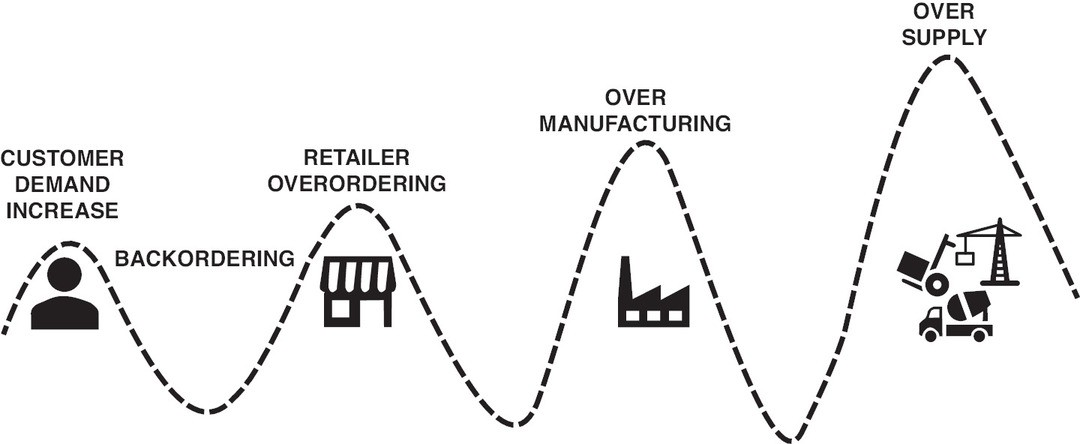
\includegraphics[width=0.9\textwidth]{../../Figures/Buoi_05A/Figure 12.1 Bullwhip Effect.jpeg}
            \caption{Hiệu ứng chiếc roi da}
        \end{figure}
    \end{columns}
\end{frame}

% Slide 10
\begin{frame}{Sự phóng đại hoảng loạn}
    \begin{itemize}
        \item Một tiếng thì thầm rất cẩn trọng của khách hàng.
        \item Qua vài bước trung gian, nó biến thành một \textbf{tiếng hét hoảng loạn} ở cuối chuỗi cung ứng.
        \item Để ngăn chặn tiếng hét này, quản trị viên cần phải dự báo được chính xác khi nào Backorder thực sự xảy ra.
    \end{itemize}
\end{frame}

% Slide 11
\begin{frame}{Tập dữ liệu mất cân bằng (Imbalanced Data)}
    \textbf{Một bài toán vô cùng hóc búa về mặt dữ liệu:}
    \begin{itemize}
        \item Tập đoàn lớn có đầy rẫy dữ liệu chuỗi cung ứng.
        \item Nhưng đứt gãy chuỗi cung ứng lại hiếm khi xảy ra.
        \item Hàng triệu đơn hàng giao trơn tru, trong khi chỉ có vài trăm đơn bị thiếu hụt.
        \item Sự chênh lệch quá lớn giữa "cái bình thường" và "cái bất thường" tạo ra Tập dữ liệu mất cân bằng.
    \end{itemize}
\end{frame}

% Slide 12
\begin{frame}{Tại sao Thống kê Truyền thống thất bại?}
    \begin{itemize}
        \item Khi đưa một tập dữ liệu mà tỷ lệ bình thường áp đảo hoàn toàn vào mô hình dự báo thống kê truyền thống, chúng sẽ \textbf{hoàn toàn vô dụng}.
        \item Khắc tinh của những tập dữ liệu phức tạp này chính là \textbf{Học Máy (Machine Learning)}.
    \end{itemize}
\end{frame}

% Slide 13
\begin{frame}{Học Máy: Cây Quyết định (Decision Tree)}
    \textbf{Khởi đầu với Cây Quyết định:}
    \begin{itemize}
        \item Một công cụ phân loại đơn giản, rẽ nhánh như một cái cây.
        \item Nó dùng các biến số đầu vào (ví dụ: Dự báo doanh số, Thời gian vận chuyển).
        \item Dựa vào các biến đó để rẽ nhánh và đưa ra dự đoán: \textit{"Đơn hàng này có bị thiếu (Yes) hay không (No)?"}
    \end{itemize}
\end{frame}

% Slide 14
\begin{frame}{Phân chia Nút gốc bằng Độ vẩn đục Gini}
    \begin{columns}
        \column{0.5\textwidth}
        \textbf{Làm sao biết biến nào dùng để rẽ nhánh tốt nhất?}
        \begin{itemize}
            \item Thuật toán tính toán \textbf{Chỉ số Gini (Gini Impurity)}.
            \item Đại diện cho "độ vẩn đục" hay độ hỗn loạn của dữ liệu. Giá trị càng thấp càng tốt.
            \item Ví dụ: Chia theo \textit{Doanh số dự báo} cho Gini thấp hơn $\Rightarrow$ Được chọn làm nút rẽ nhánh đầu tiên.
        \end{itemize}
        
        \column{0.5\textwidth}
        \begin{figure}
            \centering
            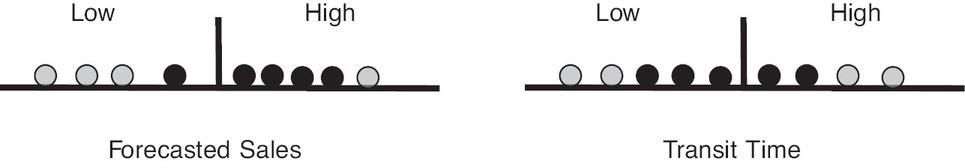
\includegraphics[width=0.85\textwidth]{../../Figures/Buoi_05A/Figure 12.3 Gini Index Calculation.jpeg}
            \caption{Tính toán Chỉ số Gini}
        \end{figure}
    \end{columns}
\end{frame}

% Slide 15
\begin{frame}{Sơ đồ Cây Phân loại (Decision Tree Splits)}
    \begin{columns}
        \column{0.4\textwidth}
        \textbf{Phân tích Cây (Hình 12.5):}
        \begin{itemize}
            \item Nút gốc đầu tiên: Doanh số dự báo (Cao/Thấp).
            \item Rẽ nhánh tiếp theo: Thời gian vận chuyển (Cao/Thấp).
            \item Đến lá cuối cùng: Kết luận Có bị Backorder hay Không.
        \end{itemize}
        
        \column{0.6\textwidth}
        \begin{figure}
            \centering
            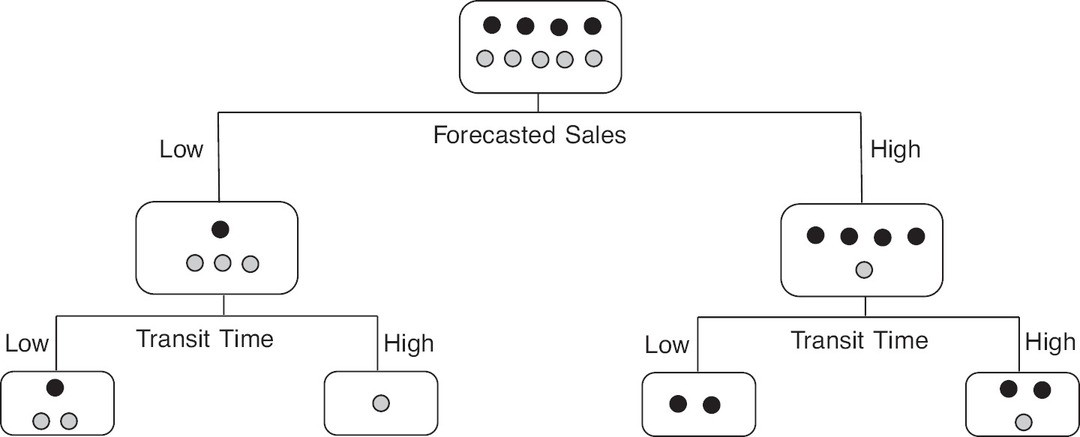
\includegraphics[width=0.9\textwidth]{../../Figures/Buoi_05A/Figure 12.5 Decision Tree Splits.jpeg}
            \caption{Sơ đồ Cây Phân loại}
        \end{figure}
    \end{columns}
\end{frame}

% Slide 16
\begin{frame}{Điểm yếu chí mạng của Cây quyết định đơn lẻ}
    \begin{alertblock}{Rất yếu ớt và Dễ bị đánh lừa!}
        \begin{itemize}
            \item Cây quyết định đơn lẻ quá \textbf{nhạy cảm}.
            \item Chỉ cần thay đổi dữ liệu huấn luyện một chút xíu, cái cây đó sẽ mọc ra những nhánh hoàn toàn khác biệt.
            \item Dẫn đến một dự đoán sai lệch ngay lập tức.
        \end{itemize}
    \end{alertblock}
    \textit{Để khắc phục sự yếu ớt này, chúng ta cần một cơ chế đột phá hơn!}
\end{frame}

% ==========================================
% SECTION 2: Rừng ngẫu nhiên & Đánh giá mô hình
% ==========================================
\section{2. Rừng ngẫu nhiên (Random Forest) \& Đánh giá Mô hình}

% Slide 17
\begin{frame}{Giải pháp đột phá: Rừng ngẫu nhiên (Random Forest)}
    \textbf{Từ một cây thành một khu rừng!}
    \begin{itemize}
        \item Thay vì phụ thuộc vào một cây quyết định mỏng manh, thuật toán Rừng ngẫu nhiên tập hợp \textbf{hàng trăm cây} lại với nhau.
        \item Nó khắc phục điểm yếu bằng 2 cơ chế đột phá:
        \begin{enumerate}
            \item Bootstrap Aggregation (Bagging).
            \item Lấy mẫu không gian con (Subspace Sampling).
        \end{enumerate}
    \end{itemize}
\end{frame}

% Slide 18
\begin{frame}{Cơ chế 1: Bootstrap Aggregation (Bagging)}
    \textbf{Đa dạng hóa góc nhìn:}
    \begin{itemize}
        \item Thay vì đưa toàn bộ dữ liệu cho tất cả các cây cùng học (chúng sẽ học giống hệt nhau).
        \item Thuật toán \textbf{bốc ngẫu nhiên} một phần dữ liệu cho một cây.
        \item Rồi lại thả vào rổ, bốc tiếp một phần khác cho cây tiếp theo.
        \item Mỗi cây sẽ được huấn luyện trên một tập dữ liệu hơi khác nhau.
    \end{itemize}
\end{frame}

% Slide 19
\begin{frame}{Cơ chế 2: Lấy mẫu không gian con (Subspace Sampling)}
    \begin{exampleblock}{Ẩn dụ: 100 Bác sĩ Hội chẩn}
        Giả sử bạn nhờ 100 bác sĩ hội chẩn cho một ca bệnh phức tạp.
        \begin{itemize}
            \item Nếu đưa cùng 1 bộ hồ sơ bệnh án đầy đủ y hệt nhau cho 100 người.
            \item Tất cả đều sẽ chỉ chăm chăm nhìn vào \textbf{triệu chứng rõ nhất} (ví dụ: ho dữ dội).
            \item Hệ quả: Cả 100 bác sĩ đều kết luận ra cùng một căn bệnh, \textbf{thiếu đi sự khách quan}!
        \end{itemize}
    \end{exampleblock}
\end{frame}

% Slide 20
\begin{frame}{Giải pháp: "Giấu bệnh án" để ép Tư duy Độc lập}
    \textbf{Làm thế nào để ép các bác sĩ suy nghĩ khác biệt?}
    \begin{itemize}
        \item Lấy mẫu không gian con hoạt động y như việc chúng ta cố tình \textbf{giấu đi} một vài kết quả xét nghiệm khi đưa cho từng người.
        \item Bác sĩ A không được xem X-quang. Bác sĩ B bị giấu chỉ số huyết áp.
        \item Khá khắc nghiệt, nhưng vô tình ép các bác sĩ (các cây quyết định) phải \textbf{suy nghĩ thực sự độc lập}.
        \item Họ buộc phải đào sâu tìm dấu hiệu bệnh lý từ các triệu chứng nhỏ nhặt, mờ nhạt hơn.
    \end{itemize}
\end{frame}

% Slide 21
\begin{frame}{Sức mạnh của Đám đông (Wisdom of the Crowd)}
    \begin{itemize}
        \item Khi tập hợp chẩn đoán của 100 bác sĩ với 100 góc nhìn hoàn toàn độc lập đó lại.
        \item Rồi lấy \textbf{bầu chọn số đông (Majority Vote)}.
        \item Chúng ta sẽ có một kết quả dự đoán chính xác và ổn định hơn gấp nhiều lần so với một cây duy nhất!
    \end{itemize}
\end{frame}

% Slide 22
\begin{frame}{Vấn đề: Dữ liệu Mất cân bằng}
    \textbf{Chúng ta quên mất một điều!}
    \begin{itemize}
        \item Dữ liệu của chúng ta vẫn cực kỳ mất cân bằng (Hiếm khi xảy ra thiếu hụt).
        \item Nếu cứ để mô hình học một cách tự nhiên từ dữ liệu, nơi mà số lần giao thành công gấp 100 lần thiếu hụt...
        \item \textbf{Mô hình Học Máy sẽ trở nên vô cùng Lười biếng!}
    \end{itemize}
\end{frame}

% Slide 23
\begin{frame}{Căn bệnh Lười biếng của Mô hình}
    \begin{block}{Quy luật "Khôn lỏi"}
        Mô hình nhận ra rằng: \textit{"Ồ, tôi chỉ cần nhắm mắt đoán bừa là KHÔNG BAO GIỜ THIẾU HÀNG, thì tỷ lệ chính xác (Accuracy) của tôi nghiễm nhiên vẫn đạt 99\%!"}
    \end{block}
    \begin{itemize}
        \item Mô hình gian lận bài thi bằng cách đánh lụi toàn bộ một đáp án.
        \item Doanh nghiệp sẽ sụp đổ vì mô hình bỏ lọt 100\% các ca thiếu hụt thực sự!
    \end{itemize}
\end{frame}

% Slide 24
\begin{frame}{Xử lý Lười biếng: Lấy mẫu giảm (Downsampling)}
    \begin{columns}
        \column{0.5\textwidth}
        \textbf{Kỹ thuật Downsampling:}
        \begin{itemize}
            \item Thuật toán chủ động \textbf{cắt bỏ bớt} lượng dữ liệu khổng lồ của nhóm giao hàng thành công.
            \item Ép tỷ lệ xuống sao cho nhóm bình thường chỉ nhỉnh hơn một chút (1.5 lần) so với ca thiếu hụt.
            \item Mô hình bị tước đi lợi thế về số lượng, bị dồn vào chân tường!
        \end{itemize}
        
        \column{0.5\textwidth}
        \begin{figure}
            \centering
            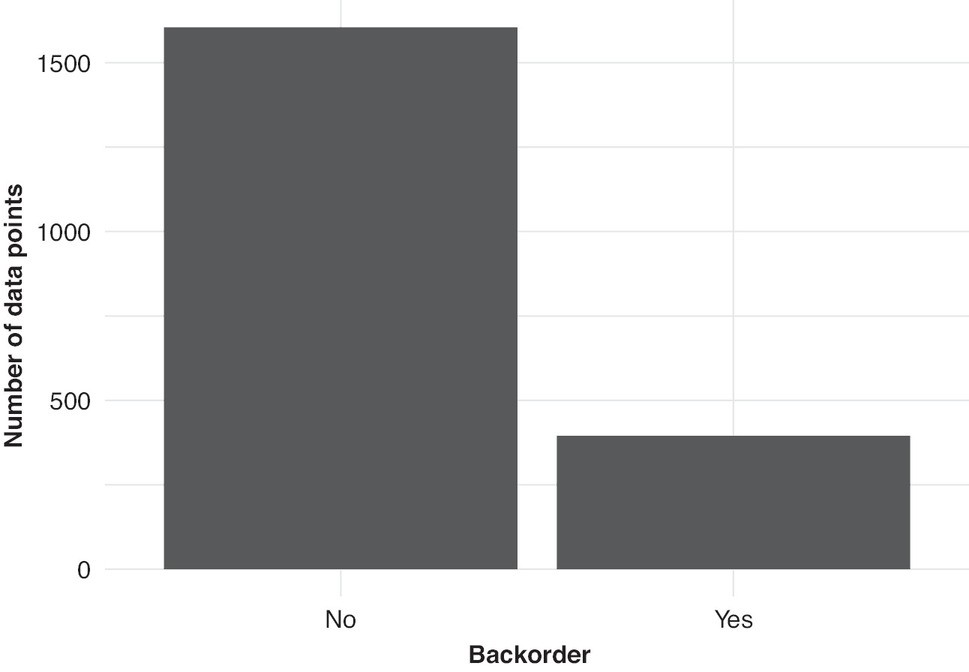
\includegraphics[width=0.9\textwidth]{../../Figures/Buoi_05A/Figure 12.6 Data Imbalance.jpeg}
            \caption{Xử lý Dữ liệu Mất cân bằng}
        \end{figure}
    \end{columns}
\end{frame}

% Slide 25
\begin{frame}{Mô hình buộc phải Học thật sự}
    \begin{itemize}
        \item Khi nhóm bình thường không còn áp đảo, đoán bừa sẽ nhận điểm 0.
        \item Mô hình buộc phải thực sự học cách nhận diện \textbf{các đặc trưng ẩn giấu} của những ca thiếu hụt thay vì chỉ gian lận.
    \end{itemize}
\end{frame}

% Slide 26
\begin{frame}{Tại sao Accuracy trở nên vô nghĩa?}
    Trong mô hình rủi ro (đứt gãy chuỗi cung ứng, gian lận thẻ tín dụng), \textbf{Độ chính xác tổng thể (Accuracy) là vô nghĩa}.
    \vspace{0.3cm}
    Chúng ta cần một bảng điểm đánh giá năng lực khắt khe hơn:
    \begin{enumerate}
        \item Độ nhạy (Sensitivity).
        \item Độ đặc hiệu (Specificity).
    \end{enumerate}
\end{frame}

% Slide 27
\begin{frame}{Đánh giá mới: Độ nhạy (Sensitivity)}
    \begin{block}{Khả năng Bắt đúng bệnh}
        \textbf{Sensitivity (True Positive Rate):} Khả năng mô hình "đánh hơi" trúng phóc những ca \textit{thực sự bị thiếu hụt hàng hóa}.
        \begin{itemize}
            \item Nếu độ nhạy thấp, mô hình sẽ \textbf{bỏ lọt tội phạm}, không cảnh báo được rủi ro đứt gãy.
        \end{itemize}
    \end{block}
\end{frame}

% Slide 28
\begin{frame}{Đánh giá mới: Độ đặc hiệu (Specificity)}
    \begin{block}{Khả năng Không báo động nhầm}
        \textbf{Specificity (True Negative Rate):} Khả năng mô hình \textit{không đưa ra những báo động giả} đối với các đơn hàng đang giao suôn sẻ.
        \begin{itemize}
            \item Nếu độ đặc hiệu thấp, mô hình sẽ gào thét báo động liên tục, khiến doanh nghiệp hoang mang và tốn kém chi phí dự phòng vô ích.
        \end{itemize}
    \end{block}
\end{frame}

% Slide 29
\begin{frame}{Bảng điểm thực sự: Đường cong ROC \& AUC}
    \textbf{Làm sao để biết mô hình có tốt không?}
    \begin{itemize}
        \item \textbf{Đường cong ROC (Receiver Operating Characteristic):} Vẽ Độ nhạy đối chiếu với (1 - Độ đặc hiệu).
        \item \textbf{Chỉ số AUC (Area Under the Curve):} Điểm số từ 0 đến 1.
        \item AUC càng gần 1, mô hình càng xuất sắc trong việc phân loại \textit{thực sự} thay vì nhắm mắt đoán bừa.
    \end{itemize}
\end{frame}

% Slide 30
\begin{frame}{Ưu điểm tuyệt vời của Rừng Ngẫu Nhiên}
    \begin{itemize}
        \item \textbf{Rất dễ tính:} Không bắt chúng ta phải chuẩn hóa dữ liệu quá cầu kỳ.
        \item \textbf{Chống nhiễu tốt:} Tự động phớt lờ đi những biến số ngoại lai nhiễu loạn (Outliers).
        \item \textbf{Kháng Đa cộng tuyến:} Xử lý rất mượt hiện tượng các biến đầu vào tác động qua lại lẫn nhau.
        \item $\Rightarrow$ Cứu cánh hoàn hảo cho môi trường hỗn loạn như chuỗi cung ứng!
    \end{itemize}
\end{frame}

% ==========================================
% SECTION 3: Phát triển sản phẩm mới & Thử nghiệm A/B
% ==========================================
\section{3. Phát triển Sản phẩm Mới \& Thử nghiệm A/B}

% Slide 31
\begin{frame}{Sự chuyển giao: Rủi ro Nội bộ}
    \textbf{Bảo vệ doanh nghiệp khỏi thế giới bên ngoài:}
    \begin{itemize}
        \item Random Forest hoạt động như cỗ máy thần kỳ để dự báo các sự điên rồ khách quan (Bão lụt, đứt gãy logistic).
    \end{itemize}
    \vspace{0.3cm}
    \textbf{Nhưng nếu nguồn cơn bất định đến từ bên trong?}
    \begin{itemize}
        \item Quyết định chủ quan của Ban giám đốc?
        \item Tung ra một giao diện app mới toanh, hay đổi cốt truyện của tựa game?
    \end{itemize}
\end{frame}

% Slide 32
\begin{frame}{Ra mắt Sản phẩm chưa từng tồn tại}
    \begin{itemize}
        \item Chúng ta \textbf{đâu có dữ liệu lịch sử} của ngày hôm qua để mà dự báo cho một sản phẩm chưa từng tồn tại!
        \item Rõ ràng, sự thay đổi bối cảnh này đòi hỏi chúng ta phải cất công cụ "dự đoán" đi.
        \item Chúng ta chuyển từ Dự báo (Predictive Modeling) sang \textbf{Thử nghiệm Nhân quả (Causal Experimentation)}.
    \end{itemize}
\end{frame}

% Slide 33
\begin{frame}{Cạm bẫy Thống kê: Tương quan \& Nhân quả}
    \textbf{Một cuộc chiến dai dẳng trong Tư duy thống kê:}
    \begin{itemize}
        \item Phân biệt giữa \textbf{Tương quan (Correlation)} và \textbf{Nhân quả (Causation)}.
        \item Đây là cạm bẫy ngọt ngào mang tên \textit{Tương quan giả tạo (Spurious Correlation)}.
    \end{itemize}
\end{frame}

% Slide 34
\begin{frame}{Tương quan Giả tạo (Spurious Correlation)}
    \begin{alertblock}{Ví dụ: Ăn kem và Cháy rừng}
        \begin{itemize}
            \item Dữ liệu cho thấy: Số lượng người ăn kem tăng lên cùng lúc với số vụ cháy rừng (Cùng di chuyển trên đồ thị).
            \item Nhưng ăn kem \textbf{không gây ra} cháy rừng!
            \item Nếu quản lý kinh doanh ra quyết định chỉ dựa trên tương quan bề mặt đó, họ đang ném tiền qua cửa sổ.
        \end{itemize}
    \end{alertblock}
\end{frame}

% Slide 35
\begin{frame}{Thiên kiến tự chọn (Self-Selection Bias)}
    \textbf{Hãy áp dụng vào thực tế kinh doanh Game:}
    \begin{itemize}
        \item \textbf{Dữ liệu chỉ ra:} Người chơi dùng Giao diện \textbf{màu Xanh} chi rất nhiều tiền mua vật phẩm so với người dùng màu Đỏ.
        \item \textbf{Kết luận sai:} Màu xanh kích thích người ta mua hàng! Ép tất cả dùng màu xanh!
    \end{itemize}
\end{frame}

% Slide 36
\begin{frame}{Sự thật về Thiên kiến tự chọn}
    \textbf{Dữ liệu đó được tạo ra như thế nào?}
    \begin{itemize}
        \item Game cho phép người chơi \textbf{được tự do chọn màu sắc}.
        \item Vô tình, những game thủ VIP bạo chi lại có gu thẩm mỹ thích màu Xanh nước biển.
        \item Màu xanh chỉ là \textit{dấu hiệu đi kèm}. Bản thân màu xanh không có "ma lực" nào thôi miên khách hàng rút ví!
    \end{itemize}
\end{frame}

% Slide 37
\begin{frame}{Giải pháp phá vỡ bẫy: Thử nghiệm A/B (A/B Testing)}
    \begin{columns}
        \column{0.5\textwidth}
        Làm sao A/B Testing phá vỡ bẫy này?
        \begin{itemize}
            \item Bằng \textbf{Sự phân bổ ngẫu nhiên (Randomization)}.
            \item Hệ thống tước đi quyền "tự chọn" của người dùng.
            \item Ném ngẫu nhiên 50\% người vào màu Xanh, 50\% vào màu Đỏ.
        \end{itemize}
        
        \column{0.5\textwidth}
        \begin{figure}
            \centering
            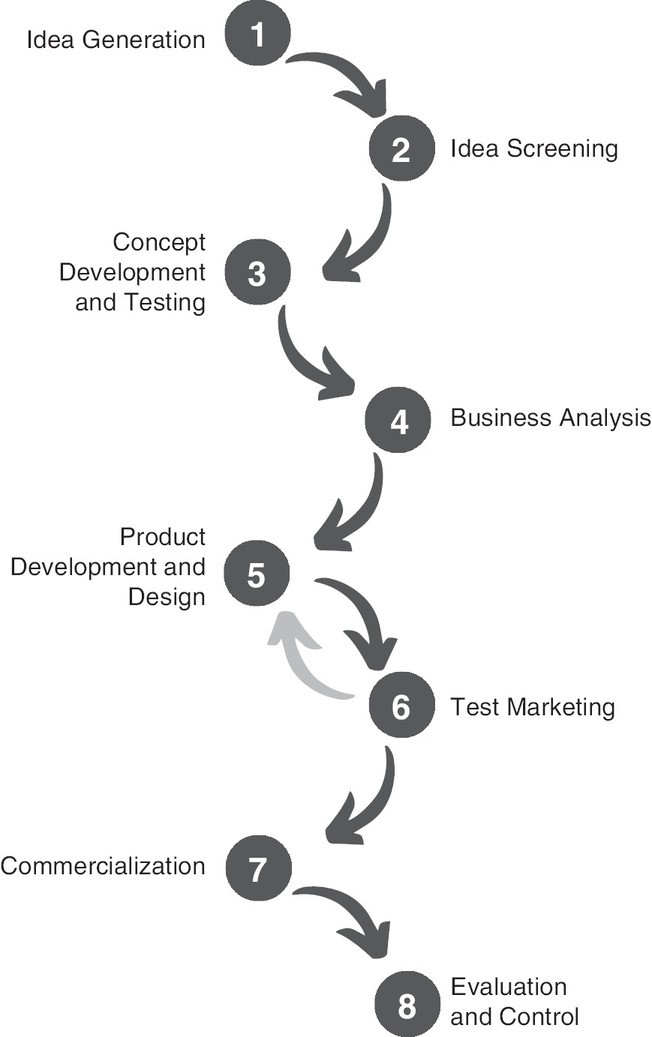
\includegraphics[width=0.9\textwidth]{../../Figures/Buoi_05B/Figure 14.1 New Product Development Process.jpeg}
            \caption{Quy trình A/B Testing}
        \end{figure}
    \end{columns}
\end{frame}

% Slide 38
\begin{frame}{Sức mạnh của Sự Ngẫu nhiên}
    \begin{itemize}
        \item Khi mẫu thử đủ lớn, sự ngẫu nhiên sẽ \textbf{cào bằng tất cả yếu tố nhiễu}.
        \item Tỷ lệ người giàu, người nghèo, lính mới, lính cũ ở cả 2 nhóm Xanh và Đỏ sẽ ngang bằng nhau chằn chặn.
        \item Mọi yếu tố bị triệt tiêu, chỉ còn lại duy nhất \textit{biến số màu sắc}.
        \item Nếu nhóm Xanh vẫn chi nhiều tiền hơn $\Rightarrow$ Ta có quyền \textbf{khẳng định Nhân quả}!
    \end{itemize}
\end{frame}

% Slide 39
\begin{frame}{Case study Game VIP: Thiết kế Nguyên mẫu}
    \textbf{Thiết kế thử nghiệm một yếu tố (One Factor Design):}
    \begin{itemize}
        \item Công ty tạo 3 nguyên mẫu Game với 3 mức độ khó: \textbf{25 (Dễ), 35 (Trung bình), 45 (Khó)}.
        \item Mục tiêu: Tìm ra mức độ khó khiến người chơi nán lại với game lâu nhất.
        \item Mỗi nhóm người chơi ngẫu nhiên chỉ tiếp xúc với một nguyên mẫu duy nhất.
    \end{itemize}
\end{frame}

% Slide 40
\begin{frame}{Giả thuyết Không (Null Hypothesis)}
    Nhưng làm sao chắc chắn sự chênh lệch thời gian chơi giữa các nhóm không phải \textbf{do ăn may}?
    \begin{block}{Gã giám khảo bảo thủ}
        Trong thống kê luôn dựng lên một rào cản gọi là \textbf{Giả thuyết Không}.
        \begin{itemize}
            \item Giống như một gã giám khảo hoài nghi khoanh tay nói: \textit{"Chẳng có mức độ khó nào tạo ra sự khác biệt cả. Mọi biến động chỉ là do ngẫu nhiên của vũ trụ!"}
        \end{itemize}
    \end{block}
\end{frame}

% Slide 41
\begin{frame}{Nhiệm vụ đập tan sự hoài nghi}
    \begin{itemize}
        \item Nhiệm vụ của khoa học dữ liệu là phải tung ra được những bằng chứng đủ mạnh để đập tan gã giám khảo đó.
        \item Với 3 nhóm trở lên, chúng ta không dùng T-test thông thường (sẽ làm tăng tỷ lệ báo động nhầm).
        \item Ta dùng \textbf{Phân tích Phương sai (ANOVA)} và \textbf{Kiểm định F (F-Test)}.
    \end{itemize}
\end{frame}

% Slide 42
\begin{frame}{Phân tích Phương sai (ANOVA) \& F-Test}
    F-Test đặt 2 thứ lên bàn cân so sánh trực tiếp:
    \begin{enumerate}
        \item \textbf{Sự khác biệt giữa các nhóm:} Cái này do sự thay đổi mức độ khó (25, 35, 45) tạo ra.
        \item \textbf{Sự khác biệt bên trong nội bộ từng nhóm:} Cái này do cá tính mỗi người chơi (Người rảnh rỗi chơi lâu, người bận rộn thoát sớm).
    \end{enumerate}
\end{frame}

% Slide 43
\begin{frame}{Cơ chế kết luận của ANOVA}
    \begin{itemize}
        \item Nếu sự chênh lệch giữa các nhóm \textbf{lớn áp đảo} so với những biến động cá nhân lộn xộn bên trong từng nhóm...
        \item Hệ thống sẽ kết luận sự chênh lệch này là \textbf{có ý nghĩa thực sự} (Statistically Significant)!
    \end{itemize}
\end{frame}

% Slide 44
\begin{frame}{Giá trị P (P-value) - Quyền lực tối thượng}
    \begin{columns}
        \column{0.5\textwidth}
        \textbf{Kết quả trả về một con số vàng:}
        \begin{itemize}
            \item Giả sử hệ thống báo Giá trị $P < 0.05$.
            \item Nghĩa là gì? Nghĩa là \textbf{xác suất để gã giám khảo bảo thủ kia đúng đã rơi xuống dưới 5\%}.
            \item Ta có đủ cơ sở khoa học để bác bỏ Giả thuyết Không!
        \end{itemize}
        
        \column{0.5\textwidth}
        \begin{figure}
            \centering
            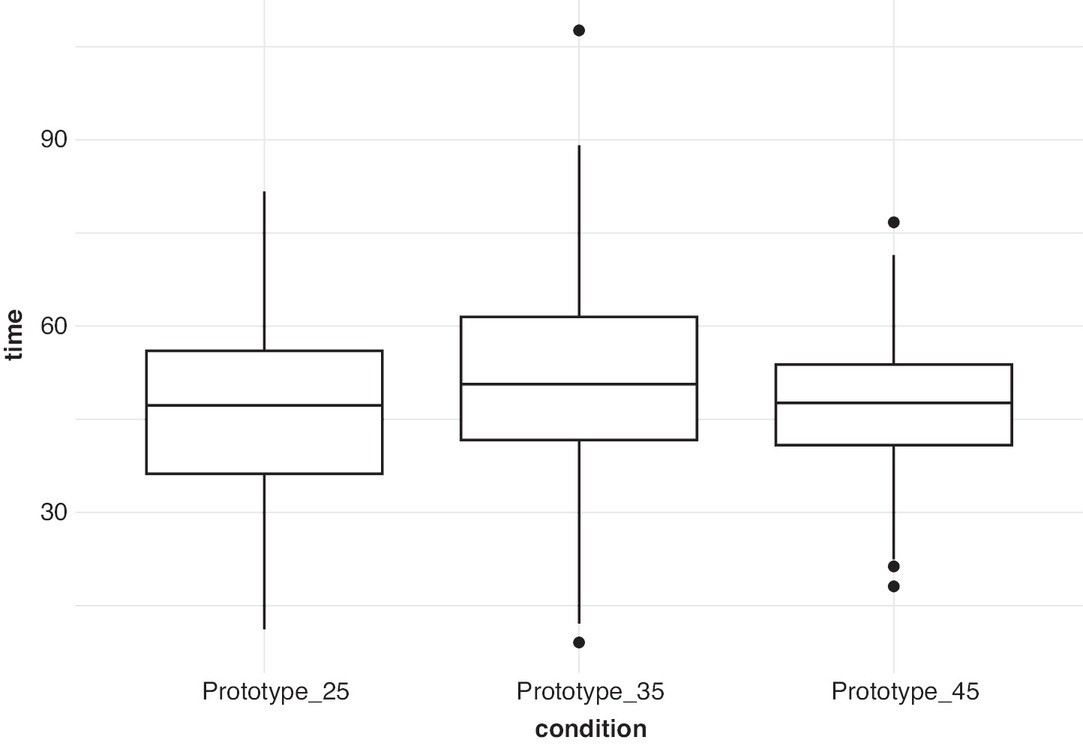
\includegraphics[width=0.9\textwidth]{../../Figures/Buoi_05B/Figure 14.2 A Boxplot of Time Spent With Different Prototypes.jpeg}
            \caption{Boxplot Thời gian tương tác}
        \end{figure}
    \end{columns}
\end{frame}

% Slide 45
\begin{frame}{Ra quyết định Tự tin}
    \begin{itemize}
        \item Khi $P < 0.05$, Công ty Game VIP không còn phải đoán mò hay cãi vã trong phòng họp nữa.
        \item Ban giám đốc có thể \textbf{tự tin 100\%} đầu tư hàng triệu đô la để tung nguyên mẫu tốt nhất (ví dụ: Mức 35) ra thị trường toàn cầu.
    \end{itemize}
\end{frame}

% Slide 46
\begin{frame}{Tổng kết: Trí tuệ nhân tạo - Tấm khiên bảo vệ vô hình}
    \textbf{Điểm chung của AI và Thống kê:}
    \begin{itemize}
        \item Dùng Rừng ngẫu nhiên để lùng sục nguy cơ đứt gãy.
        \item Dùng A/B Testing để dập tắt sự hoài nghi.
        \item Chúng hoạt động như một \textbf{Tấm khiên bảo vệ vô hình} cho doanh nghiệp.
    \end{itemize}
\end{frame}

% Slide 47
\begin{frame}{Dữ liệu không biết Tự ái}
    \begin{itemize}
        \item Tấm khiên bảo vệ doanh nghiệp khỏi quyết định cảm tính.
        \item Khỏi cái tôi quá lớn của người thiết kế luôn nghĩ mình hiểu khách hàng.
        \item Dữ liệu không biết tự ái, nó chỉ \textbf{phản ánh sự thật khách quan}.
    \end{itemize}
\end{frame}

% Slide 48
\begin{frame}{Câu hỏi Suy ngẫm}
    \begin{block}{Rủi ro bằng Không có triệt tiêu sự Sáng tạo?}
        Nếu trong tương lai, thuật toán tiến hóa hoàn hảo, mọi quyết định đều được toán học bảo chứng an toàn tuyệt đối. \\
        $\Rightarrow$ Liệu sự liều lĩnh và những ý tưởng điên rồ - thứ tạo ra các cuộc cách mạng vĩ đại - có trở nên thừa thãi?
    \end{block}
    \vspace{0.3cm}
    \textit{Đôi khi trong khoảng mịt mờ của sự bất định lại là nơi dung dưỡng cho sự sáng tạo đích thực!}
\end{frame}

% Slide 49
\begin{frame}
    \centering
    \Huge \textbf{Cảm ơn các bạn đã lắng nghe!}
    
    \vspace{0.5cm}
    \Large Hỏi \& Đáp
\end{frame}

\end{document}
